\problemname{Pickle Clicker}
\noindent

För ungefär ett halvår sedan släpptes succéspelet \emph{Pickle Clicker}. 
Efter att ha lagt otaliga timmar på spelet har Rasmus bestämt sig för att ta 
saker och ting till nästa nivå: han tänker speedrunna spelet. 

Pickle Clicker går ut på att man samlar ihop så mycket som möjligt av valutan pickles. 
Målet i en speedrun är att köpa Megapickeln så fort som möjligt, som kostar $T$ pickles. 
I spelet finns även $N$ olika typer av byggnader. De olika typerna är numrerade från 
$1$ till $N$, där den $i$:te typen producerar $p_i$ pickles per sekund och kostar 
$c_i$ pickles att bygga.

\textit{I början äger du en byggnad av typ $1$}. Varje sekund sker följande: 
\begin{enumerate}
  \item Varje byggnad du äger producerar pickles. En byggnad av typ $i$ producerar $p_i$ pickles.
  \item Därefter har du alternativet att köpa en byggnad eller köpa Megapickeln. En byggnad av typ $i$ kostar 
  $c_i$ pickles att bygga, och du måste ha råd med den för att få köpa den. Du får maximalt köpa en byggnad 
  per sekund, och det är tillåtet att ha flera byggnader av samma typ.
\end{enumerate}

Hjälp Rasmus bestämma hur han ska spela spelet så att han kan köpa Megapickeln på så få sekunder som möjligt.
Se exemplet nedan för att få en tydligare bild av reglerna.

\section*{Indata}
Den första raden innehåller heltalen $N$ och $T$ ($1 \le N \le 6$, $1 \leq T \leq 10^5$),
antalet byggnader och priset av Megapickeln.

Därefter följer $N$ rader. Den $i$:te av dessa rader innehåller heltalen $p_i, c_i$
($1 \leq p_i,c_i \leq T$), produktionshastigheten och kostnaden av byggnad $i$.

\section*{Utdata}
Skriv ut ett heltal, antalet sekunder det tar att vinna Pickle Clicker om man spelar optimalt.

\section*{Poängsättning}
Din lösning kommer att testas på en mängd testfallsgrupper.
För att få poäng för en grupp så måste du klara alla testfall i gruppen.

\noindent
\begin{tabular}{| l | l | p{12cm} |}
  \hline
  \textbf{Grupp} & \textbf{Poäng} & \textbf{Gränser} \\ \hline
  $1$    & $20$       & $N=1$ \\ \hline
  $2$    & $20$       & $T \leq 10$ \\ \hline
  $3$    & $20$       & $T \leq 1000$ \\ \hline
  $4$    & $40$       & Inga ytterligare begränsningar. \\ \hline
\end{tabular}

\section*{Förklaring av exempelfall}

\begin{figure}[h]
  \centering
  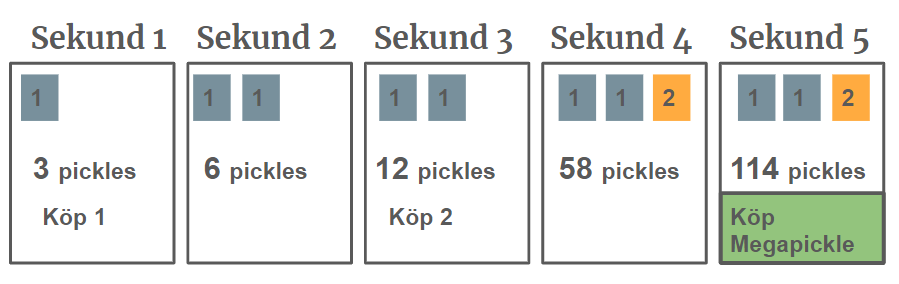
\includegraphics[width=0.7\textwidth]{sample1.PNG}
    \\Bilden visar lösningen till exempelfall 1. Den första raden beskriver vilka byggnader
    vi äger i början av motsvarande sekund. Den andra raden är hur många pickles vi har 
    efter att byggnaderna har producerat. Den sista raden indikerar om vi köper något 
    i slutet av sekunden.
  
\end{figure}
